\section{Arquitetura do sistema}


\subsection{Desenho do sistema}





\subsection{Nivel 1}

\subsubsection{Diagrama Logico}

\subsubsection{Diagrama de Implementação}

\subsubsection{Diagrama Físico} 

A figura \ref{fig:diagram-lvl1-physical} demonstra o diagrama de físico de nível 1.

\begin{figure}[h!tbp]
    \centering
    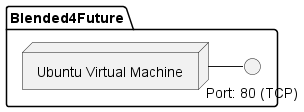
\includegraphics[width=0.5\linewidth]{capitulos/cap3-analisedoproblema/assets/arquiteturasistema/physical/physical_l1.png}
    \caption{Diagrama Físico de Nível 1}
    \label{fig:diagram-lvl1-physical}
\end{figure}





\subsection{Nivel 2}

\subsubsection{Diagrama Logico}

\subsubsection{Diagrama de Implementação}

A figura \ref{fig:diagram-lvl2-physical} demonstra o diagrama de físico de nível 2.

\subsubsection{Diagrama Físico} 
\begin{figure}[h!tbp]
    \centering
    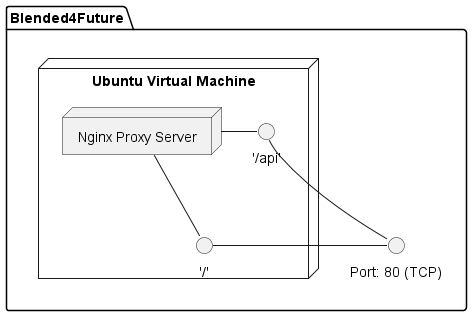
\includegraphics[width=0.6\linewidth]{capitulos/cap3-analisedoproblema/assets/arquiteturasistema/physical/physical_l2.png}
    \caption{Diagrama Físico de Nível 2}
    \label{fig:diagram-lvl2-physical}
\end{figure}


\subsection{Nivel 3}

\subsubsection{Diagrama Logico}

\subsubsection{Diagrama de Implementação}

\subsubsection{Diagrama Físico} 
A figura \ref{fig:diagram-lvl3-physical} demonstra o diagrama de físico de nível 3 

\begin{figure}[h!tbp]
    \centering
    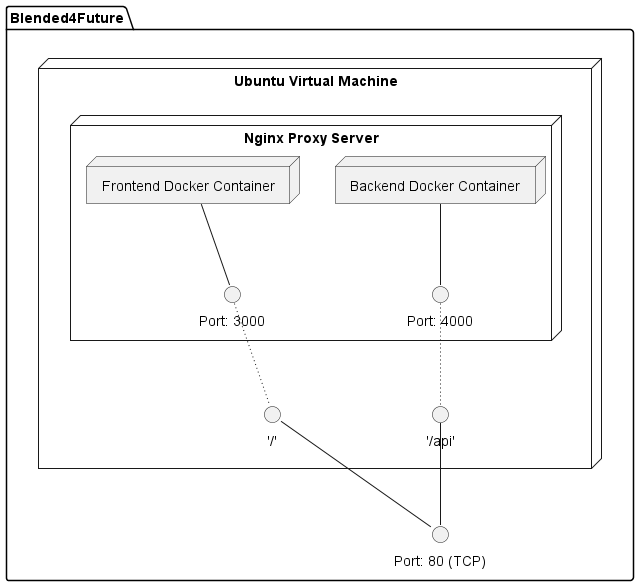
\includegraphics[width=0.7\linewidth]{capitulos/cap3-analisedoproblema/assets/arquiteturasistema/physical/physical_l3.png}
    \caption{Diagrama Físico de Nível 3}
    \label{fig:diagram-lvl3-physical}
\end{figure}





\subsection{Nivel 4 - Código}

\subsubsection{Diagrama Logico}

\subsubsection{Diagrama de Implementação}

\subsubsection{Diagrama Físico} 

A figura \ref{fig:diagram-lvl4-physical} demonstra o diagrama de físico de nível 4.

\begin{figure}[h!tbp]
    \centering
    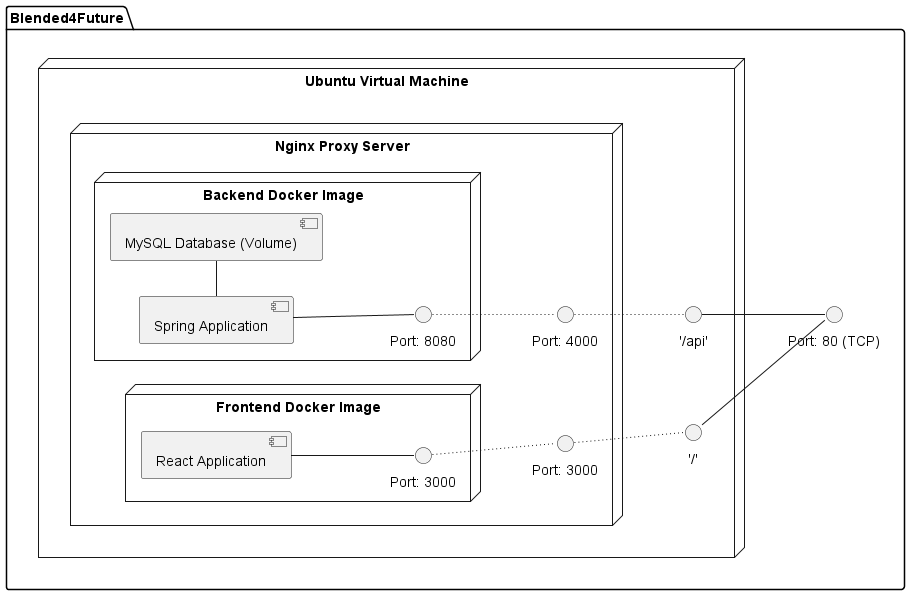
\includegraphics[width=\linewidth]{capitulos/cap3-analisedoproblema/assets/arquiteturasistema/physical/physical_l4.png}
    \caption{Diagrama Físico de Nível 4}
    \label{fig:diagram-lvl4-physical}
\end{figure}



\subsection{Padrões utilizados}
